\documentclass[12pt,a4paper]{article}
\usepackage[margin=2cm]{geometry}
\usepackage[T1]{fontenc}
\usepackage[utf8]{inputenc}
\usepackage{graphicx}
\usepackage{xcolor}
\usepackage{enumitem}
\usepackage{float}
\usepackage{caption}
\usepackage{hyperref}
\usepackage{fancyhdr}

\setlength{\parindent}{0pt}
\setlength{\parskip}{0.45em}
\setlist{nosep,leftmargin=*}
\hypersetup{colorlinks=true,linkcolor=blue,urlcolor=blue}
\pagestyle{fancy}
\fancyhead{}
\fancyfoot[C]{\thepage}

\newcounter{sectionquestion}
\newcommand{\question}[1]{\stepcounter{sectionquestion}\par\medskip\noindent\textbf{\arabic{sectionquestion}. #1}\par}
\newcommand{\proposal}[1]{\par\noindent Moj trenutni predlog: #1\par}
\newcommand{\missingmap}[2]{\begin{figure}[H]\centering\fbox{\parbox{0.86\textwidth}{\centering\vspace{1.2cm}\textbf{Karta nije uključena}\par\small #1\vspace{1.2cm}}}\caption{#2}\end{figure}}

\title{Pitanja za konsultaciju sa klimatologom\\[0.3em]\large Klimatska regionalizacija Srbije}
\author{}
\date{}

\begin{document}
\maketitle

\section{Motivacija}
\setcounter{sectionquestion}{0}

\question{Koje su prednosti Köppen--Geigerove regionalizacije? Za šta je pogodna?}
\proposal{Laka je za implementaciju i poređenje. Ima jasno tumačenje fizičkog značenja klimatskih granica. Verovatno je posebno pogodna za globalna klimatska poređenja i istraživanja klimatskih promena, na primer globalnog zagrevanja. Da li je ovo tačno?}

\question{Koji su glavni problemi Köppen--Geigerove klasifikacije u Srbiji?}
\proposal{Grupe mogu biti pregrube i prevelike za primene koje zahtevaju više detalja, kao što su urbano planiranje, zaštita biodiverziteta i poljoprivreda. Mala područja sa specifičnom klimom mogu biti uklopljena u veći region. Granice mogu biti oštre i neprilagođene lokalnim uslovima Srbije.}

\question{Šta bi naš metod trebalo da unapredi?}
\question{Ko bi mogao da koristi ovu regionalizaciju i u koju svrhu?}

\section{Pouzdanost i tačnost pomoćnih podataka}
\setcounter{sectionquestion}{0}

\question{Da li je Köppen--Geigerova mapa korišćena u radu dovoljno tačna za ovo poređenje?}

Köppen--Geigerova mapa je preuzeta iz projekta Global Hydro-Environmental Observatory (GloH2O), za klimatološki normalni period 1991--2020, sa približnom rezolucijom od 1 km. Podaci su dostupni na \href{https://www.gloh2o.org/koppen/}{GloH2O stranici sa Köppen--Geigerovim mapama}.

\begin{figure}[H]
\centering
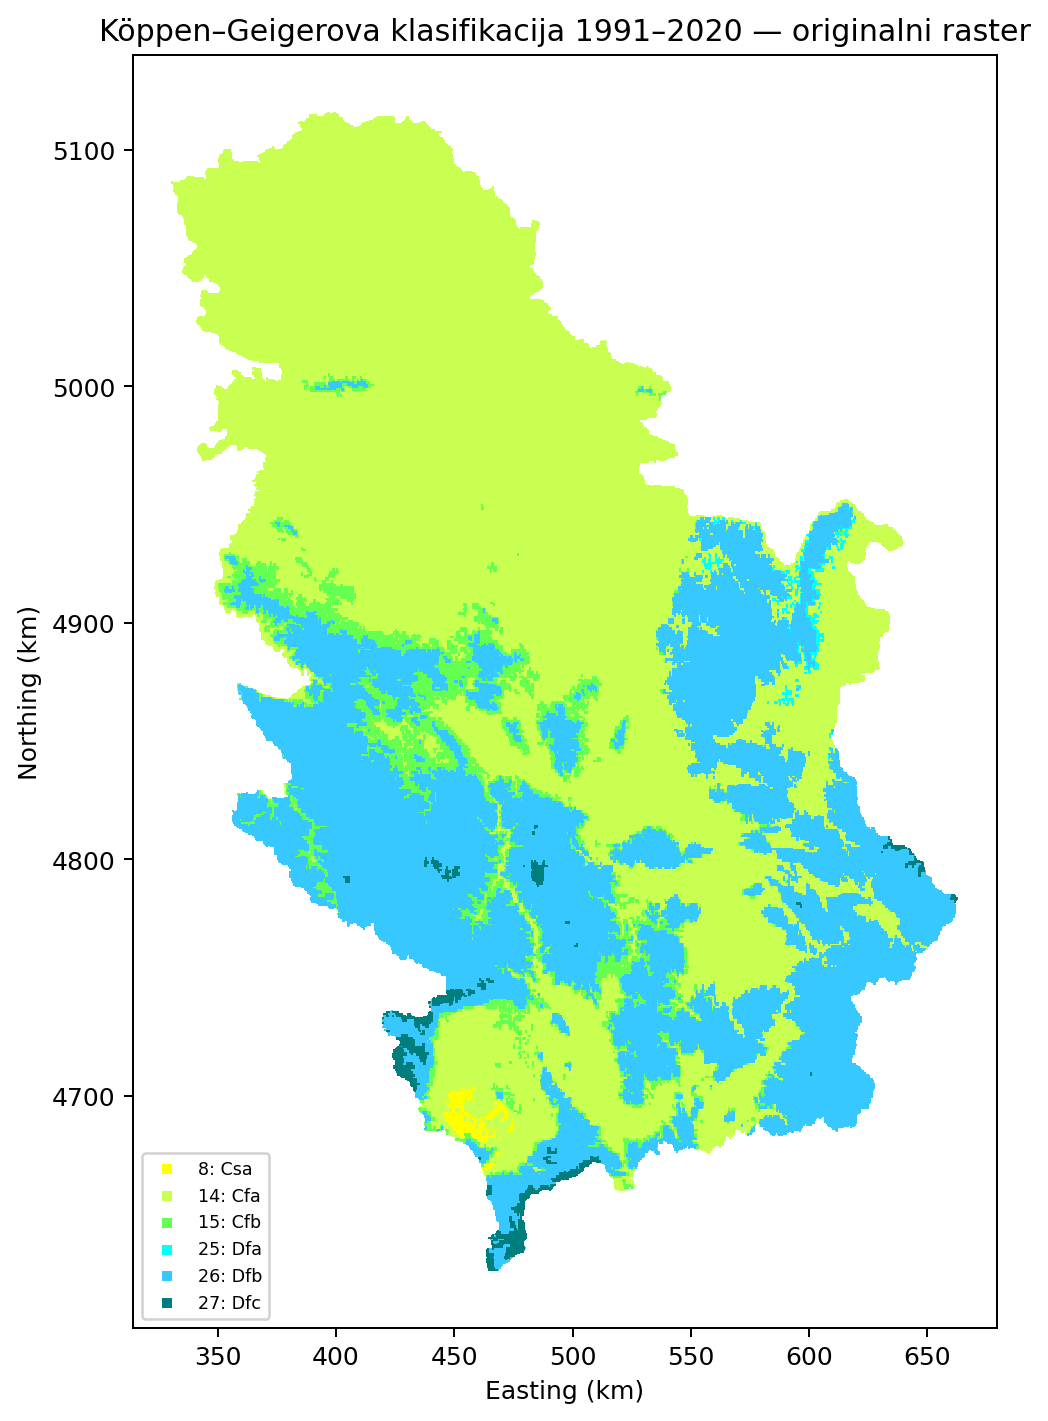
\includegraphics[width=\textwidth,height=0.70\textheight,keepaspectratio]{generated/koppen_geiger_original_srbija.png}
\caption{Köppen--Geigerova klasifikacija za Srbiju iz originalnog rastera za period 1991--2020.}
\end{figure}

\question{Da li su podaci o vegetaciji dovoljno pouzdani za validaciju?}

Podaci o zemljišnom pokrivaču potiču iz skupa CORINE Land Cover 2018, koji proizvodi Copernicus Land Monitoring Service. Korišćena je rasterska verzija rezolucije 100 m. Podaci su dostupni na \href{https://land.copernicus.eu/en/products/corine-land-cover/clc2018}{stranici CORINE Land Cover 2018}.

\begin{figure}[H]
\centering
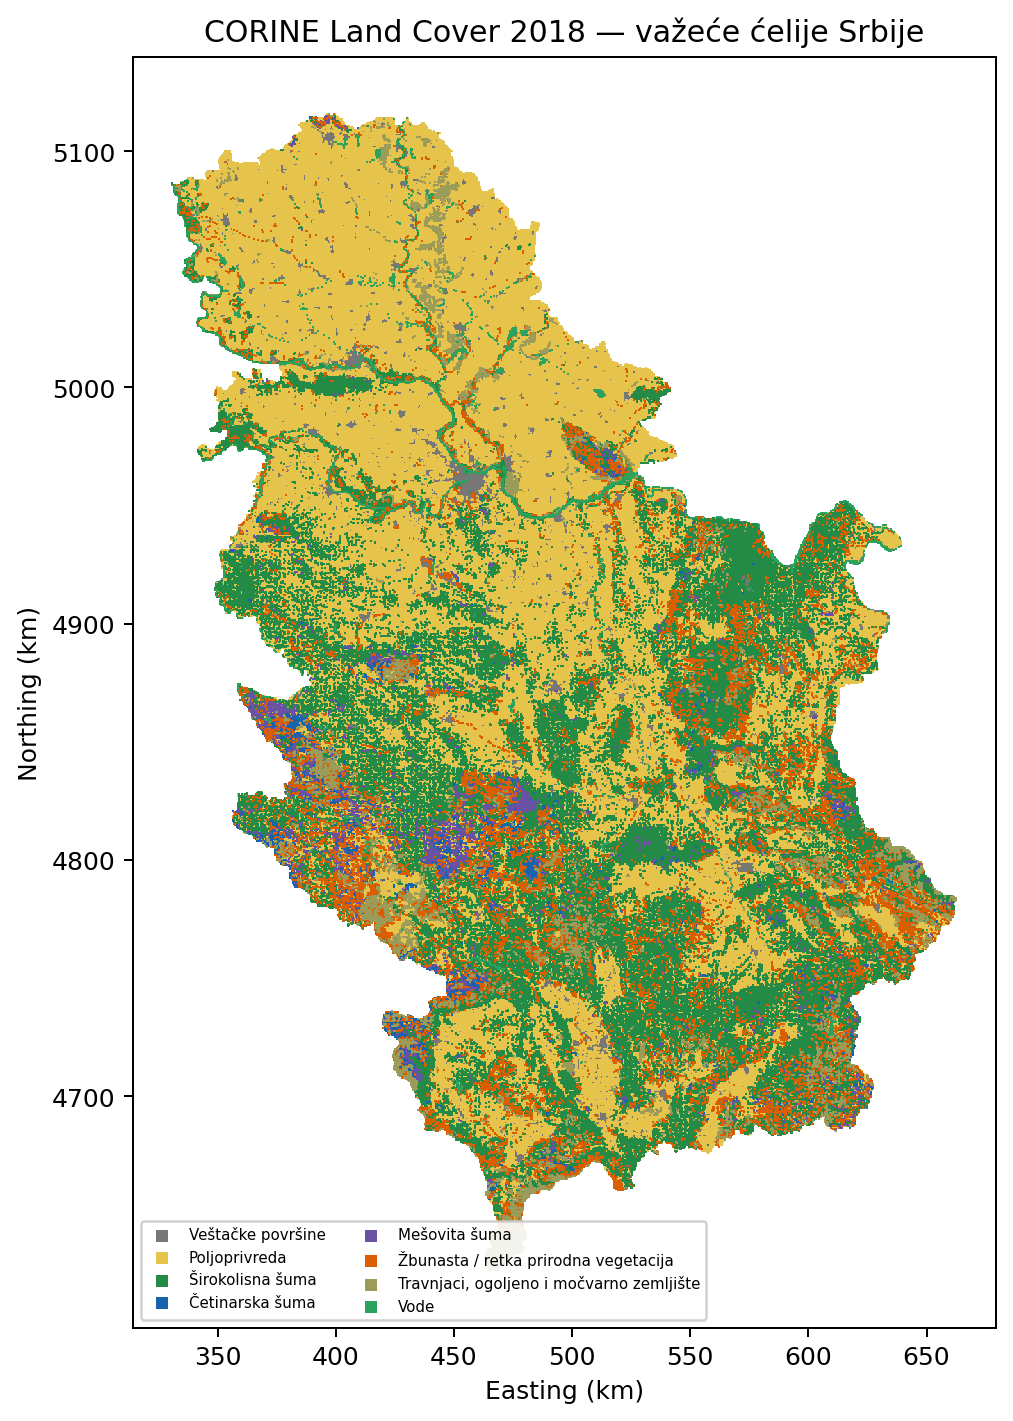
\includegraphics[width=\textwidth,height=0.70\textheight,keepaspectratio]{generated/vegetacija_srbija.png}
\caption{CORINE Land Cover 2018 prikazan kroz široke grupe korišćene u validacionoj metrici.}
\end{figure}

\textbf{Klase koje se koriste u validaciji:}
\begin{itemize}
  \item \textbf{Prirodne:} širokolisna šuma, četinarska šuma, mešovita šuma, žbunasta vegetacija, travnjaci i ogoljeno zemljište, močvare, vode.
  \item \textbf{Poljoprivredne:} nenavodnjavano obradivo zemljište, vinogradi, voćnjaci i plantaže bobičastog voća, pašnjaci, složeni obrasci obrade zemljišta, poljoprivredno zemljište sa značajnim udelom prirodne vegetacije.
  \item \textbf{Veštačke:} gradovi, putevi i druga izgrađena infrastruktura.
\end{itemize}

\question{Da li su podaci o nadmorskoj visini dovoljno pouzdani za validaciju?}

Podaci o nadmorskoj visini potiču iz skupa GEDTM30, koji je distribuiran preko platforme OpenTopography. To je model terena rezolucije 30 m, bez vegetacije i objekata. Podaci su dostupni na \href{https://portal.opentopography.org/datasetMetadata?otCollectionID=OT.082025.4326.1}{stranici GEDTM30 skupa na OpenTopography platformi}.

\begin{figure}[H]
\centering
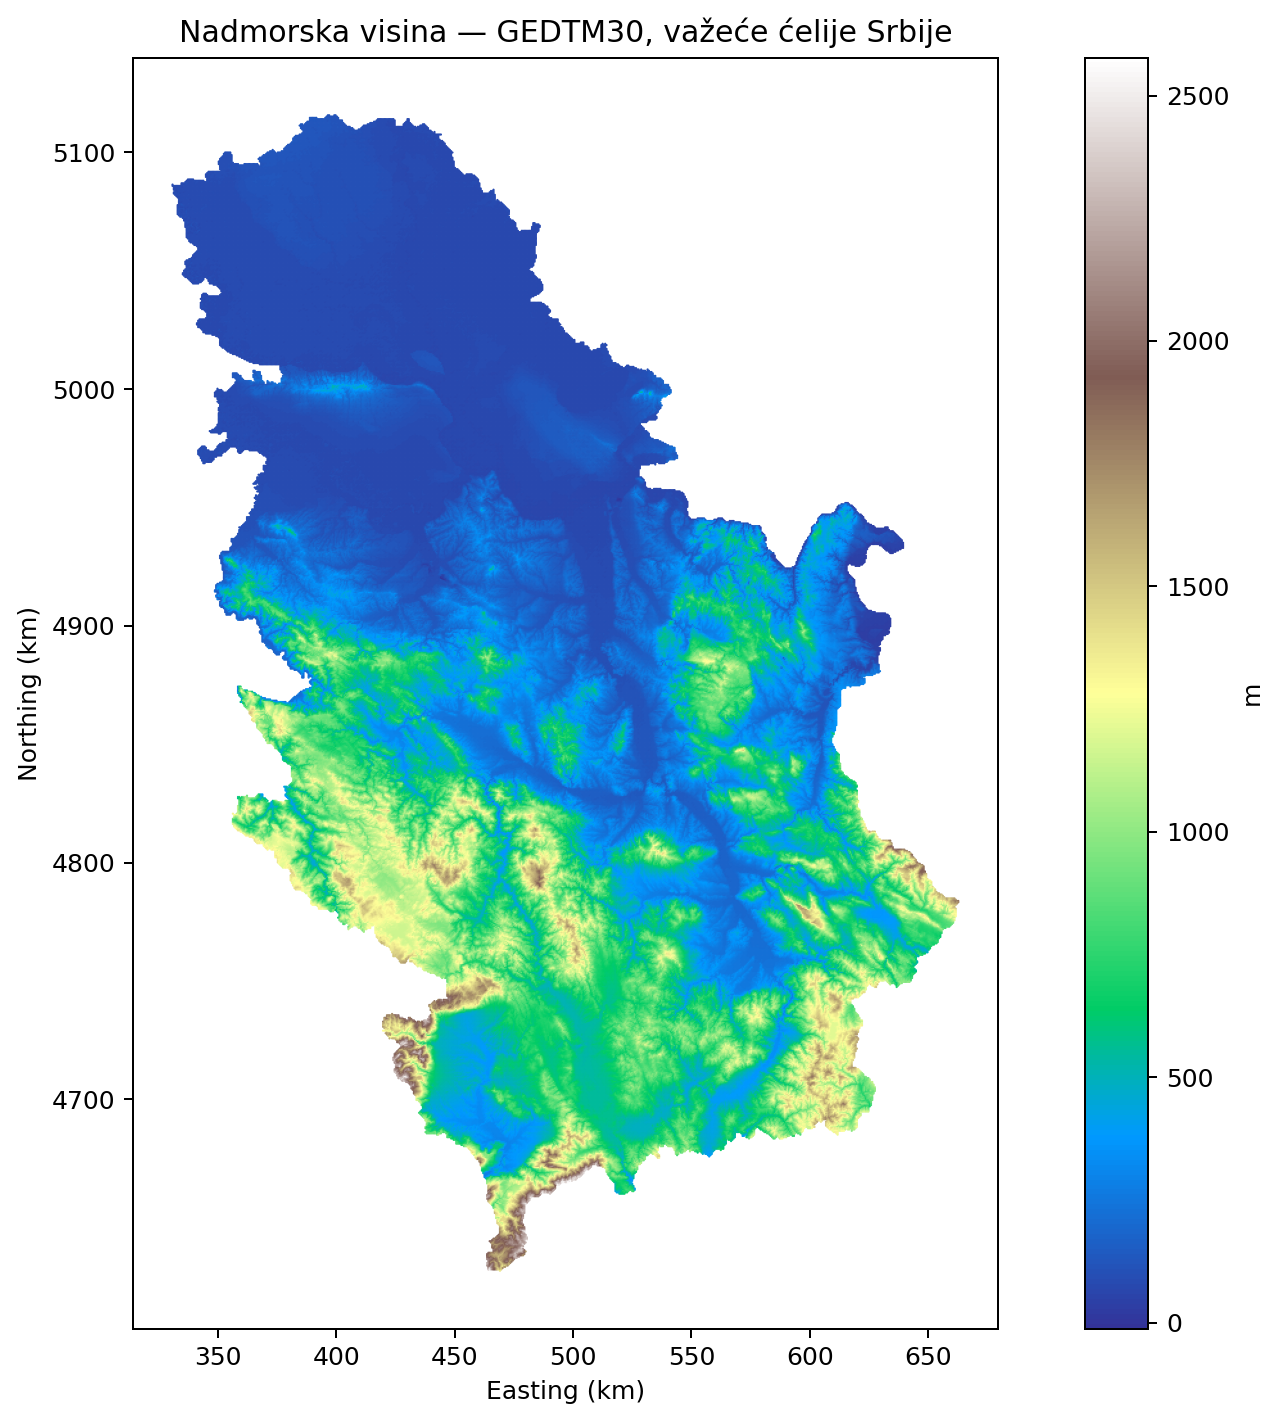
\includegraphics[width=\textwidth,height=0.70\textheight,keepaspectratio]{generated/nadmorska_visina_srbija.png}
\caption{Nadmorska visina u obuhvatu klimatske mreže, prema GEDTM30 rasteru.}
\end{figure}

\section{Očekivani rezultati}
\setcounter{sectionquestion}{0}

\question{Koliko klimatskih regiona bi bilo korisno?}
\proposal{Trenutno koristim pet regiona zato što se nakon agregacije Köppen--Geigerovih klasa dobija pet dominantnih klasa. Potrebno je proveriti da li je ovaj broj klimatski opravdan ili je izabran samo zbog poređenja sa Köppen--Geigerom.}

\question{Da li je korisnija gruba ili detaljna regionalizacija?}
\question{Kada regionalizacija postaje previše detaljna?}

\section{Analiza rezultata}
\setcounter{sectionquestion}{0}

\question{Da li regioni prikazanih rešenja imaju klimatsko značenje?}
\question{Da li odgovaraju poznatim klimatskim oblastima u Srbiji?}
\question{Da li granice regiona imaju smisla?}
\question{Da li su neki regioni očigledno pogrešni ili previše fragmentisani?}
\question{Da li su razlike u odnosu na Köppen--Geigerovu klasifikaciju značajne?}
\question{Koji rezultat bi najviše prihvatio i zašto?}

\begin{figure}[H]
\centering
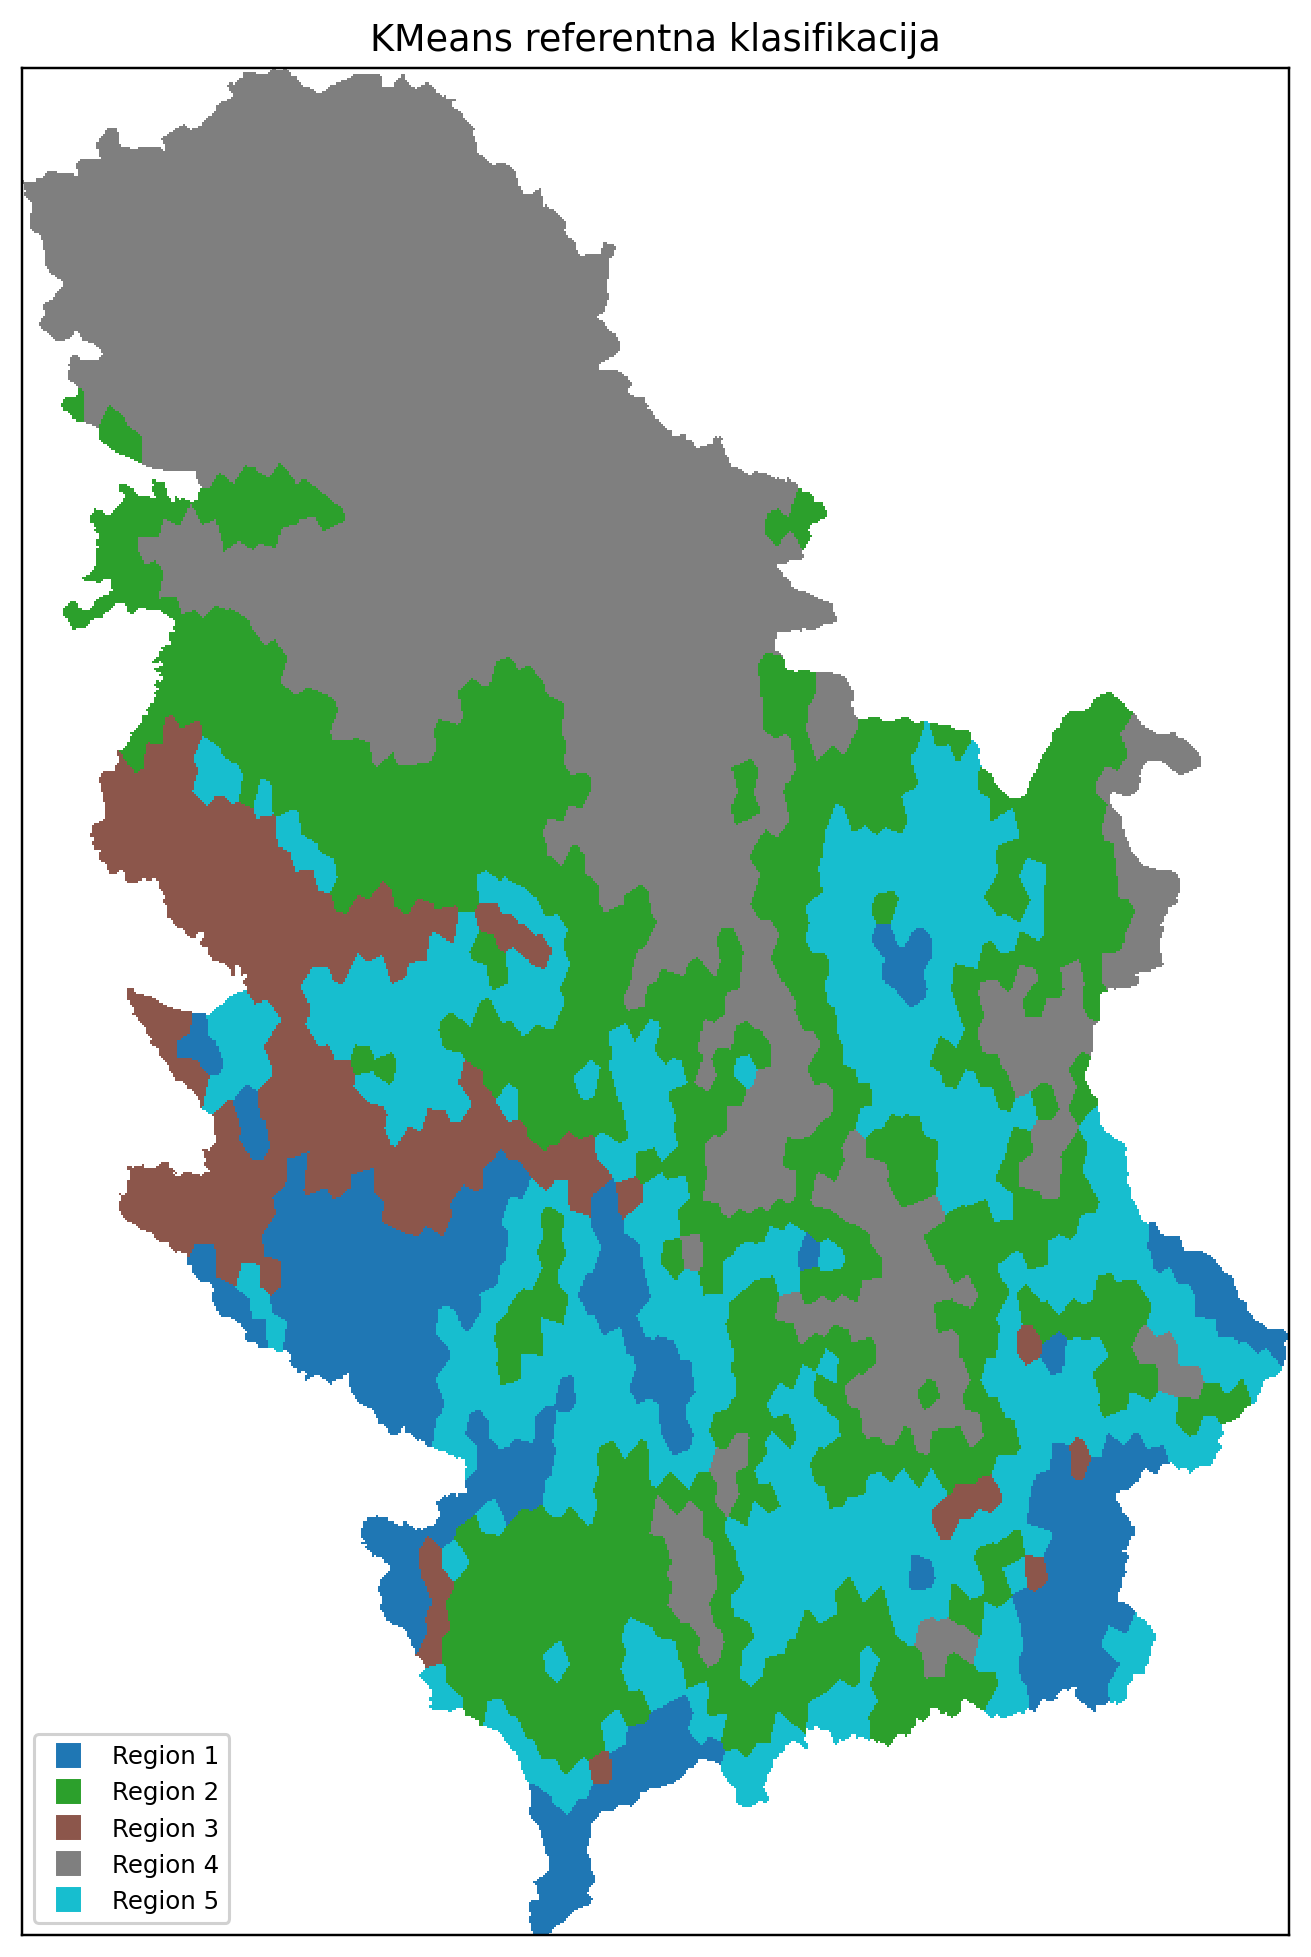
\includegraphics[width=0.68\textwidth,height=0.58\textheight,keepaspectratio]{generated/kmeans_referentna_klasifikacija.png}
\caption{KMeans kao referentna klasifikacija.}
\label{fig:kmeans-reference}
\end{figure}

KMeans je referentna metoda grupisanja lokacija prema sličnosti klimatskih osobina. Ne predstavlja predlog nove regionalizacije, već služi kao jednostavna referentna tačka za poređenje sa rezultatima metode ACO (slika~\ref{fig:kmeans-reference}).

\begin{figure}[H]
\centering
\includegraphics[width=\textwidth,height=0.82\textheight,keepaspectratio]{../experiments/results/report_comparison_outputs/selected_aco_regionalizations_koppen_features.png}
\caption{Četiri izabrane ACO regionalizacije.}
\end{figure}

\section{Mera vegetacije}
\setcounter{sectionquestion}{0}

Metrika proverava da li se unutar svakog klimatskog regiona pojavljuju slične klase zemljišnog pokrivača. Za svaki region posebno se posmatraju poljoprivredne i prirodne površine. Veštačke površine se izostavljaju jer njihov raspored više zavisi od ljudskih odluka nego od klime.

Ako region ima mali broj dominantnih klasa zemljišnog pokrivača, smatra se konzistentnijim. Ako ima mnogo različitih klasa sa sličnim udelima, smatra se heterogenijim. Poljoprivredna i prirodna konzistentnost se zatim kombinuju prema njihovom udelu u regionu. Konačna vrednost je površinski ponderisan prosek preko svih regiona. Veća vrednost znači veću konzistentnost sa zemljišnim pokrivačem.

\question{Da li ovakva mera uniformnosti vegetacije ili pokrivenosti zemljišta ima smisla za validaciju?}
\question{Da li poljoprivredne površine treba odvojiti od prirodne vegetacije pri konstrukciji validacione metrike?}
\question{Da li urbana područja treba isključiti pri konstrukciji validacione metrike?}
\question{Da li su naše grupe vegetacije preširoke ili previše detaljne?}

\section{Druge mogućnosti za validaciju}
\setcounter{sectionquestion}{0}

\question{Koje druge podatke za validaciju treba koristiti?}

\question{Da li nadmorsku visinu treba uključiti u validaciju?}
\proposal{Nadmorsku visinu trenutno koristim samo kao nezavisnu proveru, a ne kao ulaz u klasterovanje. Region sa manjom unutrašnjom varijacijom nadmorske visine smatram fizički koherentnijim.}

\end{document}
